\documentclass[a4paper,10pt]{article}
%\usepackage[latin1]{inputenc}
%\usepackage[english]{babel}
\usepackage{graphicx}
\usepackage{graphics}
\usepackage{enumerate}
\usepackage{fullpage}
\usepackage{amsmath}
\usepackage{amsfonts}
\usepackage{hyperref}
\usepackage{ifsym}
\usepackage{parskip}
\usepackage[numbers,sectionbib]{natbib}

% Egne kommandoer for enklere vektornotasjon
\renewcommand{\vec}[1]{\mathbf{#1}}
\renewcommand{\(}{\left(}
\renewcommand{\)}{\right)}
%\renewcommand{\>}{\right>}
%\renewcommand{\<}{\left<}
\newcommand{\dd}[2]{\frac{\mathrm{d}#1}{\mathrm{d}#2}}
\newcommand{\ddd}[2]{\frac{\mathrm{d^2}#1}{\mathrm{d}#2^2}}
\newcommand{\dpart}[2]{\frac{\partial#1}{\partial#2}}
\newcommand{\dpartt}[2]{\frac{\partial^2#1}{\partial#2^2}}
\newcommand{\qqq}{\qquad\qquad\qquad}
\newcommand{\f}[2]{\frac{#1}{#2}}
\newcommand{\bs}[1]{$\boldsymbol #1$}
\newcommand{\bsa}[1]{\boldsymbol #1}
\usepackage{listings}
\usepackage{color}
\usepackage{textcomp}
\definecolor{listinggray}{gray}{0.9}
\definecolor{lbcolor}{rgb}{0.9,0.9,0.9}
\lstset{
 backgroundcolor=\color{white},
 tabsize=4,
 rulecolor=,
 language=c++, 
 basicstyle=\scriptsize,
 upquote=true,
 aboveskip={1.5\baselineskip},
 columns=fixed,
 showstringspaces=false,
 extendedchars=true,
 breaklines=true,
 prebreak = \raisebox{0ex}[0ex][0ex]{\ensuremath{\hookleftarrow}},
 frame=single,
 showtabs=false,
 showspaces=false,
 showstringspaces=false,
 identifierstyle=\ttfamily,
 keywordstyle=\color[rgb]{0,0,1},
 commentstyle=\color[rgb]{0.133,0.545,0.133},
 stringstyle=\color[rgb]{0.627,0.126,0.941},
}
\usepackage{subfig}
%\usepackage{wrapfig}
\usepackage{epstopdf}

\title{Project 1 - INF5620}

\date{\today}
\author{Kand. Nr. 31}

\newenvironment{changemargin}[2]{%
 \begin{list}{}{%
 %\setlength{\topsep}{0pt}%
 \setlength{\leftmargin}{#1}%
 \setlength{\rightmargin}{#2}%
 %\setlength{\listparindent}{\parindent}%
 %\setlength{\itemindent}{\parindent}%
 %\setlength{\parsep}{\parskip}%
 }%
 \item[]}{\end{list}}
 
 \newcommand{\maxFigure}[4]{
 \begin{figure}[htp!]
 \begin{changemargin}{-3cm}{-1cm}
 \begin{center}
 %\includegraphics[width=\paperwidth + 3cm,height=\paperheight,keepaspectratio]{#2}
 \includegraphics[scale = #2]{#3}
 \end{center}
 \end{changemargin}
\vspace{-10pt}
  \caption{\textit{#1} }
  \label{#4}
 \end{figure}
 }
 
 \makeatletter
 \setlength{\abovecaptionskip}{6pt}   % 0.5cm as an example
\setlength{\belowcaptionskip}{6pt}   % 0.5cm as an example
% This does justification (left) of caption.
\long\def\@makecaption#1#2{%
  \vskip\abovecaptionskip
  \sbox\@tempboxa{#1: #2}%
  \ifdim \wd\@tempboxa >\hsize
    #1: #2\par
  \else
    \global \@minipagefalse
    \hb@xt@\hsize{\box\@tempboxa\hfil}%
  \fi
  \vskip\belowcaptionskip}
\makeatother
%%%%%%%%%%%%%%%%%%%%%%%%%%%%%%%%%%%%%%%%%%%%%%%%%%%%%%%%%%%%%
%% DOCUMENT
%%%%%%%%%%%%%%%%%%%%%%%%%%%%%%%%%%%%%%%%%%%%%%%%%%%%%%%%%%%%%
\begin{document}

\section*{Abstract}
The two dimensional wave equation can be used to model many interesting problems such as electromagnetic waves and tsunami waves. We develop a numerical solver based on an explicit scheme and discuss algorithm validation, stability, visualization and techniques for complex geometries. MayaVi is used to visualize and we have written our own visualizer using OpenGL.

\section*{Theory}
The wave equation is quite powerful in the sense that it describes many important systems in physics. We have the general equation with damping coefficient $b$, wave velocity $q(x,y)$ and source $f(x,y,t)$ given as
\begin{align}
\frac{\partial^2 u}{\partial t^2} + b\frac{\partial u}{\partial t} =
\frac{\partial}{\partial x}\left( q (x,y)
\frac{\partial u}{\partial x}\right) +
\frac{\partial}{\partial y}\left( q (x,y)
\frac{\partial u}{\partial y}\right) + f(x,y,t),
\end{align}
or more compact
\begin{align}
\frac{\partial^2 u}{\partial t^2} + b\frac{\partial u}{\partial t} =
\nabla \cdot \big(q(x,y) \nabla u \big )
\end{align}
The velocity function $q(x,y)$ describes the wave propagation speed in the point $(x,y)$. For water waves, this can be interpreted as the depth $h$ at the point $(x,y)$ as water wave velocities behave like $c(h) \propto \sqrt h$. 
\subsection*{Boundary and initial conditions}
The equation is second order in time and space, so in order to have a unique solution, we need the initial condition $u(x,y,t=0) = I(x,y)$ and its derivative $\dpart{u}{t}|_{t=0}=V(x,y)$. In addition, when the wave hits a wall, we use the boundary condition
\begin{align}
\label{eq:boundary}
\nabla u\cdot \textbf n = 0 = \dpart{u}{n}
\end{align}
where $\dpart{u}{n}$ is the derivative in the direction normal to the boundary. 

\subsection*{Standing wave}
By assuming a constant wave velocity $q(x,y)=k$, a solution to the equation is the standing wave
\begin{align*}
u(x,y,t) &= \exp(-bt)\cos\Big(\f{m_xx\pi}{L_x}\Big)\cos\Big(\f{m_yy\pi}{L_y}\Big)\cos{\omega t}\\
&= \exp(-bt)\cos (k_x x)\cos (k_y y)\cos{\omega t}
\end{align*}
for arbitrary integers $m_x$, $m_y$ and frequency $\omega$. This solution gives a rather messy source term $f(x,y,t)$, but it's trivial to calculate. We rewrite the solution to $u(x,y,t) = T(t)\cdot R(x,y)=T(t)\cdot X(x) \cdot Y(y)$
\begin{align*}
b\dd{T}{t} &= -e^{-bt}(b^2\cos \omega t + b\omega \sin \omega t)\\
\ddd{T}{t} &= e^{-bt}\Big[(b^2 - \omega^2)\cos\omega t + 2b\omega\sin\omega t\Big] \\
\ddd{X}{x} &= - k_x^2 X(x)
\end{align*}
The left hand side of the wave equation now reads
\begin{align*}
e^{-bt}R(x,y)&\Big[ (b^2 - \omega^2)\cos\omega t + 2b\omega\sin\omega t -b^2\cos \omega t - b\omega \sin \omega t \Big]\\
& = e^{-bt}R(x,y)\Big[-\omega^2\cos\omega t + b\omega\sin\omega t\Big]\\
& = u(x,y,t)\Big[-\omega^2 + b\omega\tan\omega t\Big]
\end{align*}
Which gives
\begin{align*}
u(x,y,t)\Big[-\omega^2 + b\omega\tan\omega t\Big] = -q\big[ k_x^2 + k_y^2 \big]u(x,y,t) + f(x,y,t)
\end{align*}
We can solve this for the source term
\begin{align*}
f(x,y,t) &= u(x,y,t)\Big[ k^2 - \omega^2 + b\omega \tan\omega t\Big]
\end{align*}
where $k^2=q(k_x^2 + k_y^2)$. If we choose this as the source term, we only need to calculate the first time derivative to have a unique solution.
\begin{align*}
V(x,y) &= \dpart{u(x,y,t)}{t}\Big|_{t=0} \\
& = -e^{-bt}(b\cos\omega t + \omega \sin\omega t)\cos(k_xx)\cos(k_yy)\Big|_{t=0}\\
&= -b\cos(k_xx)\cos(k_yy)
\end{align*}
The initial condition is 
\begin{align*}
I(x,y) &= u(x,y,t=0) = \cos(k_xx)\cos(k_yy)
\end{align*}
We will use this solution in one of the verifications later.
\section*{Numerical implementation}

\subsection*{Discretization}
If we look at a system of widths $L_x$ and $L_y$, we can divide the system into a grid with $N_x\times N_y$ points where we have the steplengths $\Delta x=\f{L_x}{N_x-1}$ and $\Delta y=\f{L_y}{N_y-1}$. The wave function $u$ is now represented as a matrix $u_{i,j}$ where $u_{i,j}=u(x_i,y_j)$ in each timestep $t_n$. The numerical wave equation can be discretized on operator form
\begin{align*}
\Big[D_tD_t u + bD_{2t}u = D_x  q[D_x u] + D_y q [D_y u]\Big]^n_{i,j}
\end{align*}
where we have applied the standard approximation for second derivatives in time, the centered difference scheme on the first derivative and the Crank-Nicolson twice in the spatial part. Written out in full index form, this evaluates to
\begin{align*}
\text{L.H.S. } & = \f{u^{n+1}_{i,j} + u^{n-1}_{i,j} - 2u^{n}_{i,j}}{\Delta t^2} + b\f{u^{n+1}_{i,j}-u^{n-1}_{i,j}}{2\Delta t}\\
\text{R.H.S. } & = \f{1}{\Delta x}\Bigg(q_{i+\f{1}{2},j}\Bigg[\f{u^n_{i+1,j} - u^n_{i,j}}{\Delta x}\Bigg]
- q_{i-\f{1}{2},j}\Bigg[\f{u^n_{i,j} - u^n_{i-1,j}}{\Delta x}\Bigg]\Bigg)\\
&+\f{1}{\Delta y}\Bigg(q_{i,j+\f{1}{2}}\Bigg[\f{u^n_{i,j+1} - u^n_{i,j}}{\Delta y}\Bigg]
- q_{i,j-\f{1}{2}}\Bigg[\f{u^n_{i,j} - u^n_{i,j-1}}{\Delta y}\Bigg]\Bigg)
\end{align*}
This can be solved for $u_{i,j}^{n+1}$ and we can easily evolve the system in time. We notice that to calculate timestep $n+1$, we need both timesteps $n$ and $n-1$ because of the second derivative in time. This reflects the requirement of both $u(x,y,t=0) = I(x,y)$ and $u(x,y,t+\Delta t)$ as mentioned above. There are two standard ways to calculate the second timestep $u(x,y,0+\Delta t)$. If we have the initial condition $\dpart{u}{t}|_{t=0}=0$, we apply the forward difference scheme
\begin{align*}
\f{u^{+1}_{i,j} - u^{0}_{i,j}}{\Delta t} = 0\\
\end{align*}
which gives
\begin{align*}
u^{+1}_{i,j} = u^{0}_{i,j}
\end{align*}
for all $i,j$. If we have the more complicated and general system where $\dpart{u}{t}|_{t=0} = V(x,y)$, we can use the centered difference scheme and define
\begin{align*}
\f{u^{+1}_{i,j} - u^{-1}_{i,j}}{2\Delta t} = V(x_i,y_j)\\
\end{align*}
which gives
\begin{align*}
u^{-1}_{i,j} = u^{+1}_{i,j} + V_{i,j}
\end{align*}
where we evaluate $V_{i,j} = V(x_i,y_j)$. We can again solve the equation for $u_{i,j}^{+1}$ by using only one timestep. The second derivative in the spatial dimensions also require both neighbor points which will give problems at the boundaries where such points might not exist. We solve this by using \eqref{eq:boundary} and apply the centered difference scheme on $\dpart{u}{n}$, assuming that the normal vector is in either the $x$- or $y$-direction and define
\begin{align*}
\dpart{u}{x} = 0 = \f{u^n_{i+1,j} - u^n_{i-1,j} }{ 2\Delta x}
\end{align*}
which again gives
\begin{align}
\label{eq:boundary2}
u^n_{i-1,j} = u^n_{i+1,j}
\end{align}
These points are often called ghost points, or ghost cells, because they don't really exist.

\subsection*{More general boundary conditions}
If we have walls at the boundaries $u_{i,j} | i,j \in \{0,N_x-1\}$, we can easly do an if-test and apply \eqref{eq:boundary2}. The code will then be rather messy with special cases for each boundary, and the systems geometry is limited. We can instead introduce the wall matrix $W \in \mathbb B ^{N_x\times N_y}$ where $\mathbb B$ is the boolean domain. Each point $W_{i,j}$ contains either a \textit{true} or \textit{false} value defining if that point is a wall or not. To implement this method, we have the matrices $u\_$ and $u\_prev\_$ which contains all the values of $u$ in the two previous timesteps. In addition we have the wall matrix $W$ with booleans. When we access the elements $u_{i\pm 1,j}$ or $u_{i,j\pm 1}$, we create a function that returns the elements $u_{i\mp 1,j}$ or $u_{i,j\mp 1}$ if there is a wall at the respective point. The algorithm looks like
\begin{lstlisting}
int idx(int i) {
	return (i+10*Nr)\%Nr;
}

double u(int i,int j, int di, int dj) {
	if(W(idx(i+di),idx(j+dj))) {
		return u_(idx(i-di),idx(j-dj));
	} 

	return u_(idx(i+di),idx(j+dj));
}
\end{lstlisting}

\subsection*{Complex objects and varying $q(x,y)$}
By using the method above we can represent more complex objects and geometries by filling the wall matrix $W$ instead of making complicated special cases programmatically. One way to handle both boundary conditions and the wave velocity field $q(x,y)$ is to use BMP-images to represent the geometry of the system. If we create a black-and-white BMP-image of size $N_x\times N_y$ pixels, this can in our program be represented as a matrix $G \in \mathbb R ^{N_x\times N_y}$ where each value $G_{i,j} \in (0,1)$ containing the white level value in that point. This image can be used to define both boundaries (walls and objects) and ground (wave velocity) by choosing a threshold value $p$ such that $W_{i,j} = G_{i,j} \geq p$. By shifting the values $G_{i,j} \rightarrow G_{i,j}-p$, the value in $G$ can now be interpreted as the depth where values above zero will behave like hard boundaries and values below zero will affect the wave velocity.

\begin{lstlisting}
void calculateWalls() {
	for(int i=0;i<Nx;i++) {
		for(int j=0;j<Ny;j++) {
			walls(i,j) = ground(i,j) >= 0;
		}
	}
}
\end{lstlisting}
\begin{figure}[htp]
\centering
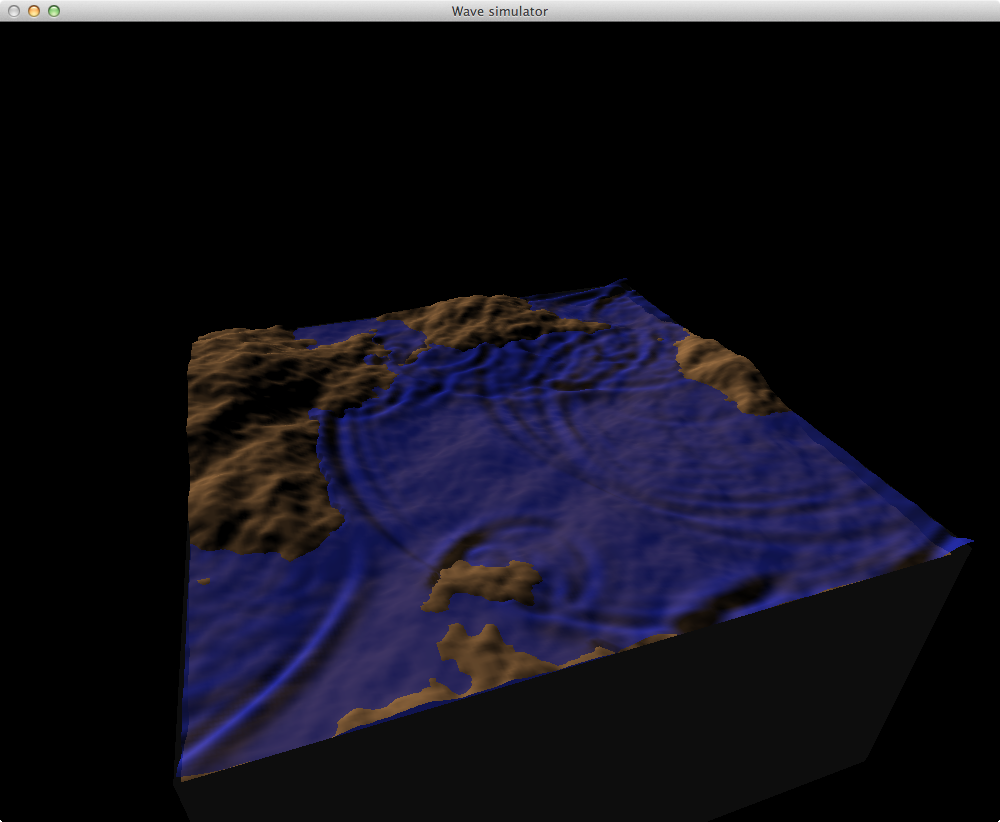
\includegraphics[width=13cm]{reflection.png}
\caption{Waves that are reflected by the boundaries, e.g. the mountains.}
\label{fig:reflection}
\end{figure}

\subsection*{Source term and rain}
One application of source terms can be raindrops falling into the water. We can create raindrops randomly at a height $z_0$ and let them fall with constant velocity. Once a raindrop hits the surface, $z_{i,j} \leq u_{i,j}$, we increase the source term $f_{i,j}$ by a suitable value, we used 0.005.
\begin{lstlisting}
void moveRainDrops() {
    for(int k=0;k<raindrops.size();k++) {
        raindrops[k].z -= 0.005;

        if(raindrops[k].z <= u_(raindrops[k].i,raindrops[k].j)) {
            source(raindrops[k].i,raindrops[k].j) = 0.01;
            raindrops.erase(raindrops.begin()+k--);
        }
    }
}
\end{lstlisting}
This creates those beautiful ripples we expect from raindrops hitting the surface. Usually there are a lot of raindrops, so in figure \ref{fig:rain}, we see that the water surface is quite noisy.
\begin{figure}[htp]
\centering
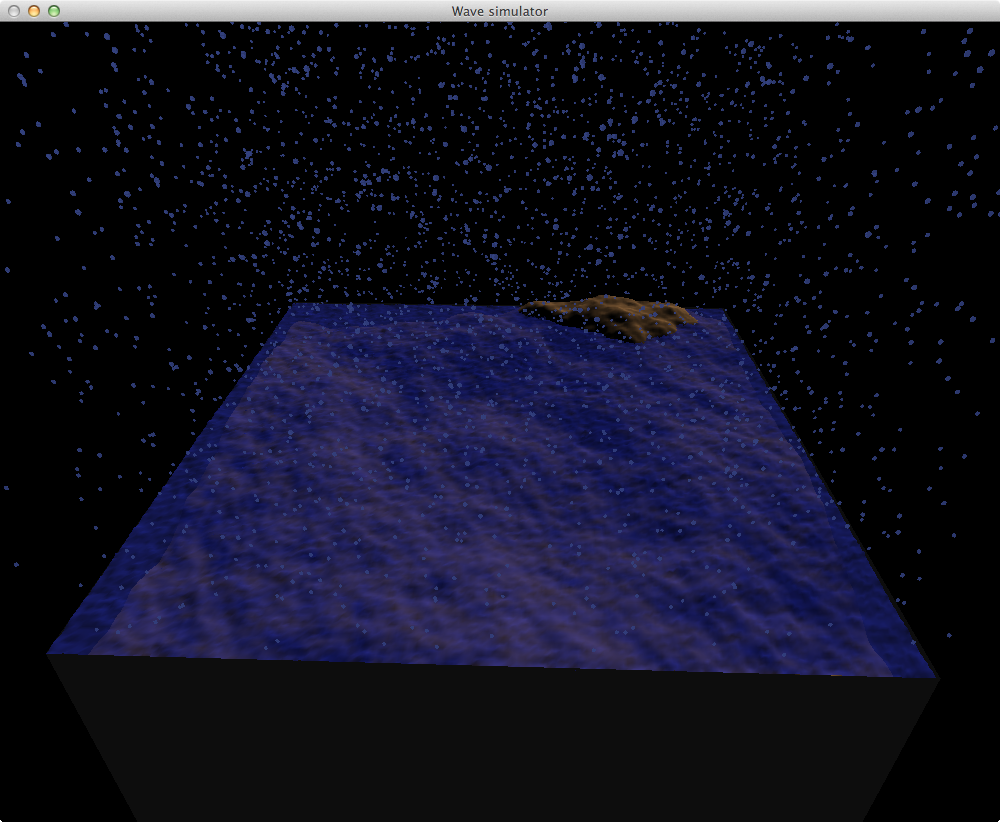
\includegraphics[width=13cm]{rain.png}
\caption{Raindrops creating a lot of ripples that add up to noisy surface.}
\label{fig:rain}
\end{figure}

\section*{Verification}
In order to make sure the solver is free of bugs, we need to run it through some test solutions. Natural choices that should be reproduced exactly is the constant solution (for instance, $u(x,y,t) = 1.2$) and a plug wave. For python based programs, these tests can be put into a nosetest module, and done in \verb nose_test_betterwave.py  which can be found in the project folder. We there let each test run over all versions of the code (scalar, vectorized and (ideally) c++). For a constant solution we may create an initial state by
 \begin{lstlisting}[language=Python]
def I(x, y):
	return 1.2
 \end{lstlisting}
and test the output of the solver, $u$, through for instance:
\begin{lstlisting}[language=Python]
u_exact = 1.2*np.ones((Nx+1,Ny+1))
diff = np.abs(u_exact - u).max()
nt.assert_almost_equal(diff, 0, delta=1E-14)
\end{lstlisting}

 For the plug wave, we can do a very similar test, as long as we make sure the wave travels for exactly, and integer number of periods, so that the wave in the exact same state as it was initially. In the nosetest module this was done by trial and error while using a relatively coarse grid. We made the initial state by the function
  \begin{lstlisting}[language=Python]
def I(x, y):
		return np.logical_and((np.abs(x) < Lx/2.+1), (np.abs(x) > Lx/2.-1))*1.
 \end{lstlisting}
and test the output of the solver, $u$, through for instance:
\begin{lstlisting}[language=Python]
x = np.linspace(0, Lx, Nx+1)  # mesh points in x dir
y = np.linspace(0, Ly, Ny+1)  # mesh points in y dir
X,Y = np.meshgrid(x,y)
u_exact = I(X,Y)
T = 1.0
n = int(T/dt - 5)
fname = 'solution_%06d.txt' % n
u = np.loadtxt(fname)
diff = np.abs(u_exact - u[:,0]).max()
nt.assert_almost_equal(diff, 0, delta=1E-14)
\end{lstlisting}
 where the suitable value for $n$ had to be found manually.

Once these tests are passed, we began looking at the convergence rate of the solvers. In order to do this, we note in theory, the error in the solution should to lowest order behave as 
\begin{equation}\label{eq:errororder}
 E = C_1 (\Delta x)^2 + C_2(\Delta y)^2 + C_3(\Delta t)^2
\end{equation}
So that if we double the amount of mesh points in both time and space, we should reduce the error by a factor of 4. In order to measure the error, we decided to run the solver up to a given time (for simplicity, $T = 1.0$), and compare the solution to the exact solution some manufactured function in each point $(x_i,y_j)$. If we denote this error by $e_{i,j}$, then a reasonable expression for the total error would be 
\begin{equation}\label{eq:errorestimate}
 E = \left( \frac{1}{N_x N_y}\sum_{i,j} e_{i,j}^2 \right)^{1/2}.
\end{equation}
And so we check if this error is reduced by roughly a factor 4 if we double the number of grid points. Since this is only an estimate of the error behavior we will need to be a bit gentle on this requirement, and so we should check that the ratio between consecutive errors is, for instance, 1/4 up to an accuracy of $\pm 0.05$. We decided to test this on the standing wave solution 
\begin{equation}
 u(x,y,t) = e^{-bt}\cos\left(\frac{m_x \pi x }{L_x}\right)\cos\left(\frac{m_y \pi y }{L_y}\right)\cos(\omega t)
\end{equation}
with source and initial state as described earlier. A test for convergence rate may look something like
\begin{lstlisting}[language=Python]
mx = 4.; my = 4.; b = 0.01; omega=np.pi;
def u_exact(x,y,t):
	return ...
def f(x,y,t):
	return ...
def I(x, y):
	return ...
def V(x,y):
	return ...
Nx = 40; Ny = 40; T = 1.0
dt = 0.01
for version in ['vectorized']:
	errorlist=[0,0,0]
	for i in range(3):	
		... # construct the X-Y-grid, load the last step from file
		u_ex = u_exact(X,Y,T2)
		error = np.sqrt(np.sum((u_ex-u)**2)*dx*dy)
		errorlist[i] = error
		Nx = Nx*2;
		Ny = Ny*2;
		dt = dt/2
ratio1 = errorlist[1]/errorlist[0]
ratio2 = errorlist[2]/errorlist[1]
nt.assert_almost_equal(ratio1, 0.25, delta=0.05)
nt.assert_almost_equal(ratio2, 0.25, delta=0.05)
\end{lstlisting}

After some debugging, the program was able to successfully pass all tests for both the scalar and vectorized version.

\section*{C++ implementation}
One of our extensions is to solve the given 2d wave problem by using C++ and its (almost) bult-in libraries std and boost. This is as simple as coding the problem in python,
as the syntax of the numerics is identical. One difference is that we have to use scalar programming as a vectorized form 
puts requirements on all called functions (e.g. double sin(double x) must be rewritten/overloaded to take a matrix as argument and also return a matrix). This is not a viable approach, but scalar programming
done correctly should also be quite readable as the numerics become very close to the mathematics.

We wrote most of the code directly in main(). This could easily be converted into a general class solver, but this requires a lot of assignment code and was not done for simplicity.
Also, most of the parameters are hardcoded and can be changed at the top of main(). The various input functions (i.e. I(x,y), V(x,y), q(x,y,t) and f(x,y,t)) can also be set at this point by assigning
the general function pointers to point to the relevant functions.

We implemented the solver by using the boost::numeric::ublas::matrix template class for the matrices. This removes the need for explicit double pointer 'arithmetics' in addition to manual memeory allocation and deallocation.
The syntax is easy
\begin{lstlisting}
 matrix<double> u(Nx, Ny); // create an Nx by Ny matrix
 u(0,6) = 5; // set element (0,6) equal to 5.
\end{lstlisting}
The contrast from double pointers is obvious u(i,j) $\equiv$ u[i][j]. The matrix class also overloades the arithmetic operators (+,-,*,/), thus allowing vectorized syntax
\begin{lstlisting}
 matrix<double> u(Nx, Ny);
 matrix<double> v(Nx, Ny);
 ...
 u = u + v - 2*v;
\end{lstlisting}
This is not used in our code.

\section*{C++ parallelization}
An additional extension is to parallelize our implementation. We did this by using OpenMP, which is an API that supports shared memory multiprocessing in C, C++ and Fortran. 

Our implementation is to some extent easily parallelizable. From the numerics, we note that all calculations in a given timestep are idependent of each other. That is, for a given n, all
calculations are only dependent on the previous timestep, n-1
\begin{align*}
\rm u_{\rm n} = \rm u_{\rm n }(\rm i, \rm j, u_{n-1}).
\end{align*}
This implies that the nested spatial loop is embarrassingly parallel. In OpenMP the parallelization is done by a pragma directive
\begin{lstlisting}
// time loop
for (int n=1; n<Nt; n++) {
  // space loops
  #pragma omp parallel for
  for (int i=0; i<Nx; i++) // <-- this is parallelized
    for (int j=0; j<Ny; j++) // <-- all threads run this loop for all j
      unext(i,j) = ... something only dep. on n-1 ...
}
\end{lstlisting}
This code forks the outer spatial loop into $N_{\rm cores}$ threads, where $N_{\rm cores}$ is the number of CPU cores. The threads eavenly (if possible) divide the i interval [0,Nx) into $N_{\rm cores}$ 
intervals.
At the end of the i-loop, the slave threads terminate and only the master thread continues execution. Since all threads share the same memory, the variables (declared before the loop) used by all threads are the same.
We could try to parallelize the innermost loop (i.e. the j-loop) instead, but this would probably decrease the efficiency since the threads would then be created/killed for each iteration of i (compared to each n), 
thus creating more overhead.

\subsection*{Speedtests}
To check the efficiency of the parallelized code, we tried a few runs with and without parallelization. We use the following spatial domains:� $50 \times 50$, $100 \times 100$, $400 \times 400$. The time used (in seconds) 
by each run is given in table \ref{tbl1}.
\begin{table}[h!]
   \begin{tabular}{| c || l | l |  l|}
    \hline 
    \# cores & 50x50 & 100x100 & 400x400 \\ \hline \hline
    1 & 0.89 & 3.54 & 57.1 \\ \hline 
    4 & 0.5 & 0.97 & 15.3\\ \hline  \hline 
    Ratio & 1.8 & 3.65 & 3.73 \\ \hline
   \end{tabular}
      \caption{\label{tbl1} Execution time as a function of number of cores and spatial domain.}
\end{table}
If the entire algorithm was completely parallelizable the ratio has an obvious theoretical maximum ratio of $N_{\rm cores}$. We can see that the parallel code is about $3.7$ times faster, which is lower than the theoretical
maximum. This must be so, since the algorithm has not been fully parallelized. Also, we see that the ratio falls with decreasing spatial domain size, which is probably due to increased overhead from 
thread creation/destruction compared to the gain from parallelization. Larger spatial domain should increase the ratio even further, as this overhead becomes more and more negligible.
\section*{Error convergance}
We are given an exact solution to the 2d wave equation (1) in the project text. In this section, we study the numerical approximation of this solution. The derivations of $I(x,y)$, $V(x,y)$ and $f(x,y,t)$ are
given in the section above. 

There are various ways to calculate the error of the approximation. We wanted to check the dependence of the error in spatial resolution, $\Delta x$ and $\Delta y$. 
We take $\Delta x = \Delta y \equiv h$ ($F_x = F_y = 1$) and $\Delta t = 0.1h$ ($F_t = 0.1$) to ensure stability. To calculate the error, we use equation \ref{eq:errorestimate} in the following form
\begin{align}
 E = h \sqrt{\sum_{i,j}(u_{i,j} - u^{\rm exact}_{i,j})^2}.
 \label{eq123}
\end{align}
We expect $E/h^2$ to be constant
\begin{align*}
 E &= C_t \Delta t^2 + C_x \Delta x^2 + C_y \Delta_y^2 \\
 &= C_t F_t^2 h^2 + C_x F_x^2 h^2 + C_y F_y^2 h^2 \\
 &= (C_t F_t^2 + C_x F_x^2 + C_y F_y^2)h^2 \\
 &\equiv Ch^2.
\end{align*}
\subsection*{Tests}
The error can readily be calculated in the code, using \ref{eq123}, at a given (nonzero) time, e.g. $T=1$. The results for various values of $h$ are listed in table \ref{tbl2}.
\begin{table}[h!]
   \begin{tabular}{| l || l | l|}
    \hline 
    $h$ & E & $E/h^2$ \\ \hline \hline
    $0.08 $ & 0.0179 & 2.80 \\ \hline 
    $0.04 $ & 0.00437 & 2.73 \\ \hline 
    $0.02$ & 0.00107 & 2.68 \\ \hline 
    $0.01$ & 0.000266 & 2.66  \\ \hline 
    $0.005$ & $6.62 \times 10^{-5}$ & 2.65 \\ \hline 
    $0.004$ & $4.23 \times 10^{-5}$ & 2.65 \\ \hline 
   \end{tabular}
   \caption{\label{tbl2} Error for given $h$ at $T=1$.}
\end{table}
We see that the factor $E/h^2$ is approximatly constant ($\approx 2.7$), as expect from error analysis. If we decrease $h$ by a factor of 2 the error decreases by a factor of $2^2 = 4$. The nosetest for this is described
above. The fact that the error behaves as expected is evidence that our implementation is correct.

\section*{Visualization}
\subsection*{MayaVi}
For a 3-dimensional animation, the standard matplotlib-library in Python shows a poor performance, with unacceptible speeds. In order to get sufficiently fast real-time animation, as well as a large improvement in speed for saving animations, we decided to animate our solutions with the MayaVi library. Using this we were able to plot solutions at a useful speed. Saving animations was done by saving the individual frames plotted by mayavi, and turning the set of pictures into an animation using the program Mencoder. Saving animations was still painfully slow, as MayaVi is not very efficient at saving plots. It turned out that, using built-in MayaVi function, one could store the picture as a set of pixel values. This set could then be plotted and saved in Pylab for an overall noticable speedup in movie creation. The details of this was stored in the function \verb mcrtmv(frames,dt,Lx,Ly,Nx,Ny,savemovie=False,mvname='test')  which can be found in the source code in the module of the same name. An screenshot of 
a plotted and stored solution can be found in figure \ref{fig:mayavitest} and several stored animations can be found among the source files. 
\\
\\
Removed the mayavitest.png since it is not in repo.
\\
\\
%\begin{figure}
%\centering
%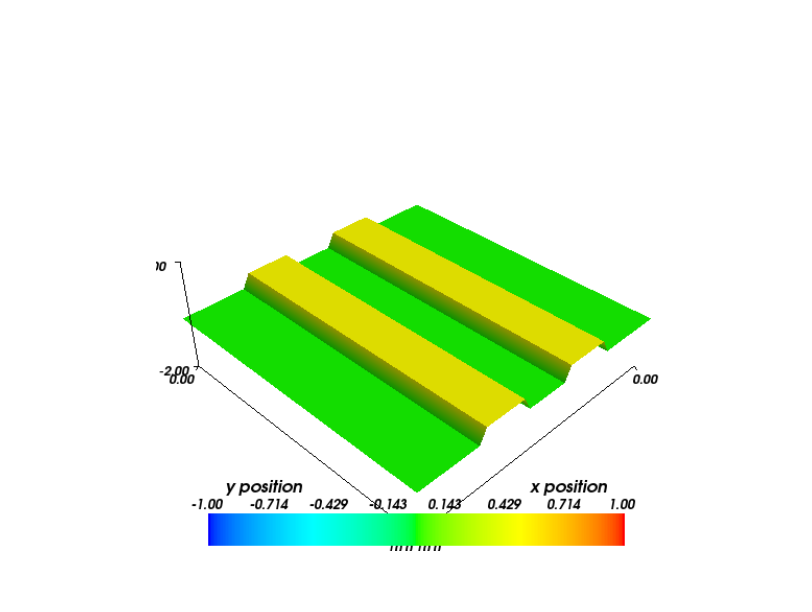
\includegraphics[width=13cm]{mayavitest.png}
%\caption{The figure shows a screenshot of a stored animation of the plug wave solution}
%\label{fig:mayavitest}
%\end{figure}

\subsection*{OpenGL}
OpenGL (Open Graphics Library, OGL) is an API that can be used to communicate with the graphics card. In a basic OGL-program, we define a window that has a width and height (measured in pixels). We are offered a set of objects or \textit{primitives} (points, triangles, quads, polygons etc) that can be rendered in the window by OGL.
\subsection*{Rendering points and triangles}
We can render a set of points at positions $r_i=(x_i,y_i,z_i)$ saved in a matrix with the following code
\begin{lstlisting}
glBegin(GL_VERTEX);
for (int i=0; i<10; i++) {
   glVertex(points[n].x,points[n].y,points[n].z);
}
glEnd();
\end{lstlisting}
Usually we want to render surfaces rather than points, so we use one of the other primitives such as \textit{GL\_TRIANGLES}. If we call \textit{glBegin(GL\_TRIANGLES);} instead, OGL expects three points defining a triangle, a \textit{face}. We can then render our whole grid by dividing it into small triangles. Rendering code might then look like
\begin{lstlisting}
glBegin(GL_TRIANGLE);
for (int i=0; i<n_faces; i++) {
   for(int j=0;j<3;j++) {
      glVertex(faces[i].points[j].x,faces[i].points[j].y,faces[i].points[j].z);
   }
}
glEnd();
\end{lstlisting}
The grid will be triangulated like we see in figure \ref{fig:triangulation1}.

\begin{figure}
\centering
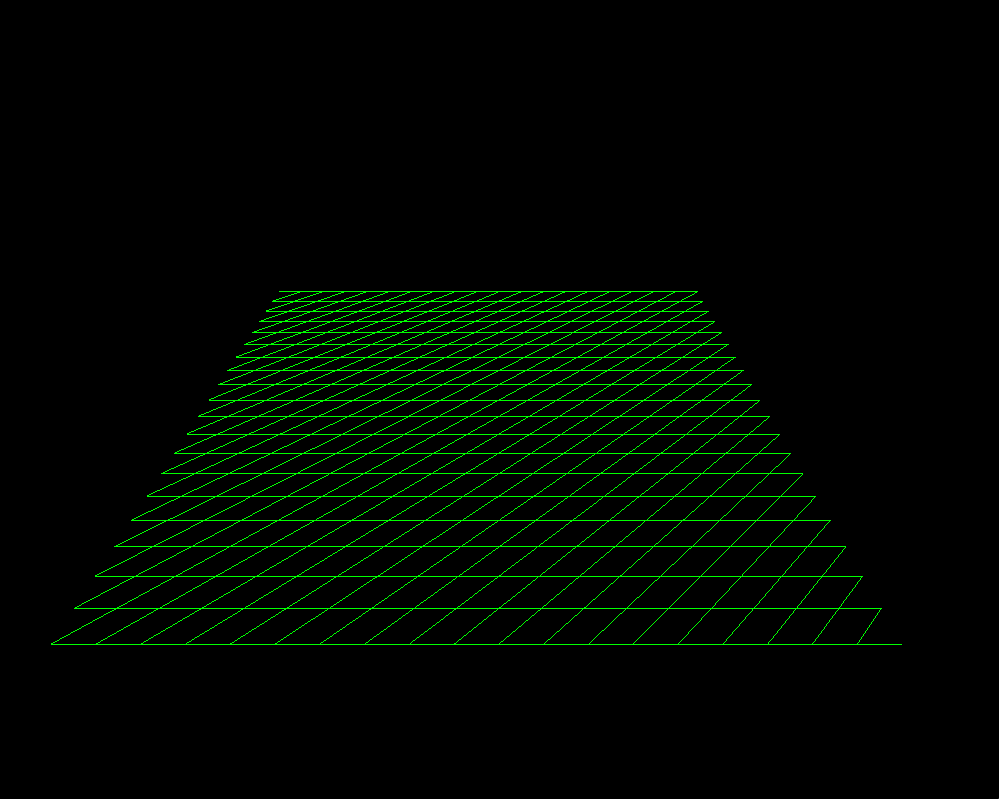
\includegraphics[width=13cm]{triangulation1.png}
\caption{Triangulation of a 20x20 grid.}
\label{fig:triangulation1}
\end{figure}

\begin{figure}
\centering
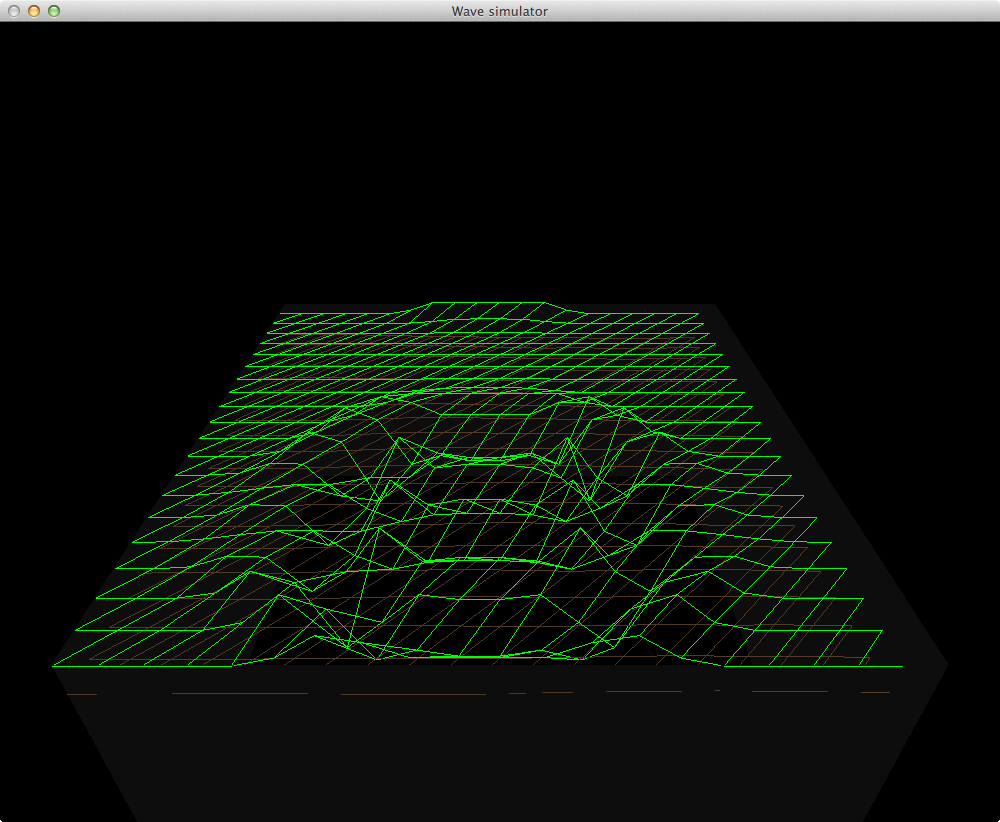
\includegraphics[width=13cm]{triangulation2.png}
\caption{Triangulation of a 20x20 grid with a wave.}
\label{fig:triangulation2}
\end{figure}

\begin{figure}
\centering
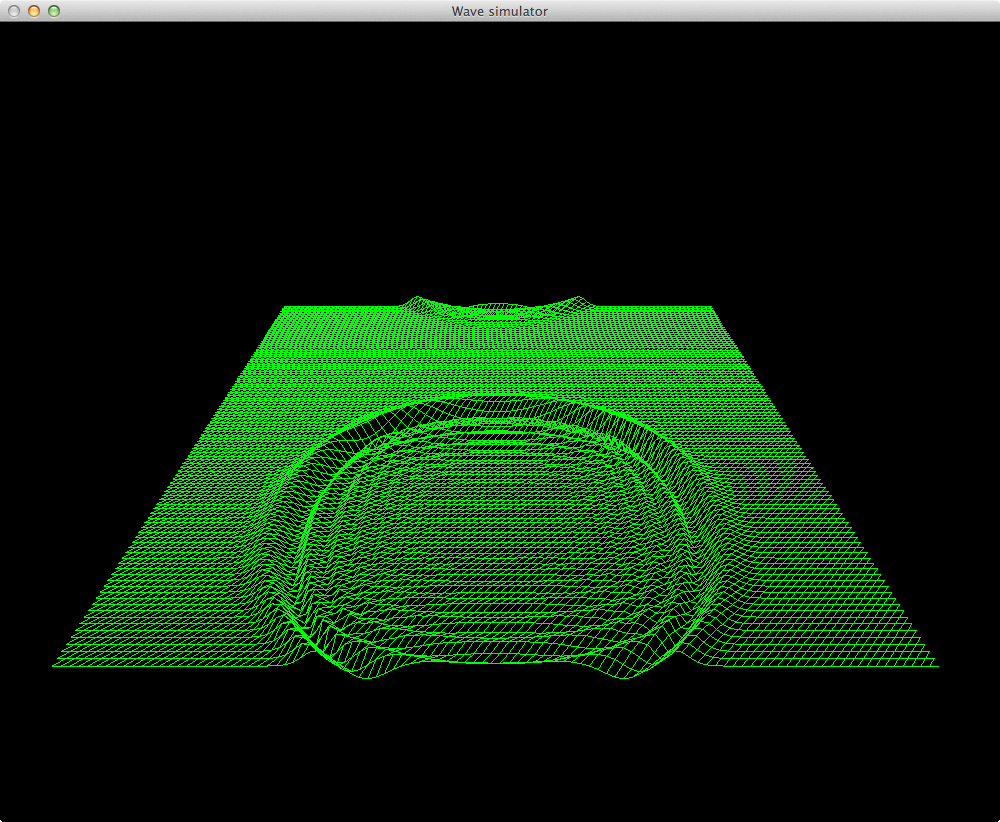
\includegraphics[width=13cm]{triangulation3.png}
\caption{Triangulation of a 100x100 grid with the same wave as in figure \ref{fig:triangulation2}.}
\label{fig:triangulation3}
\end{figure}
By increasing the grid size, the triangles get smaller and smaller and we won't even notice that there isn't a smooth surface.
\begin{figure}
\centering
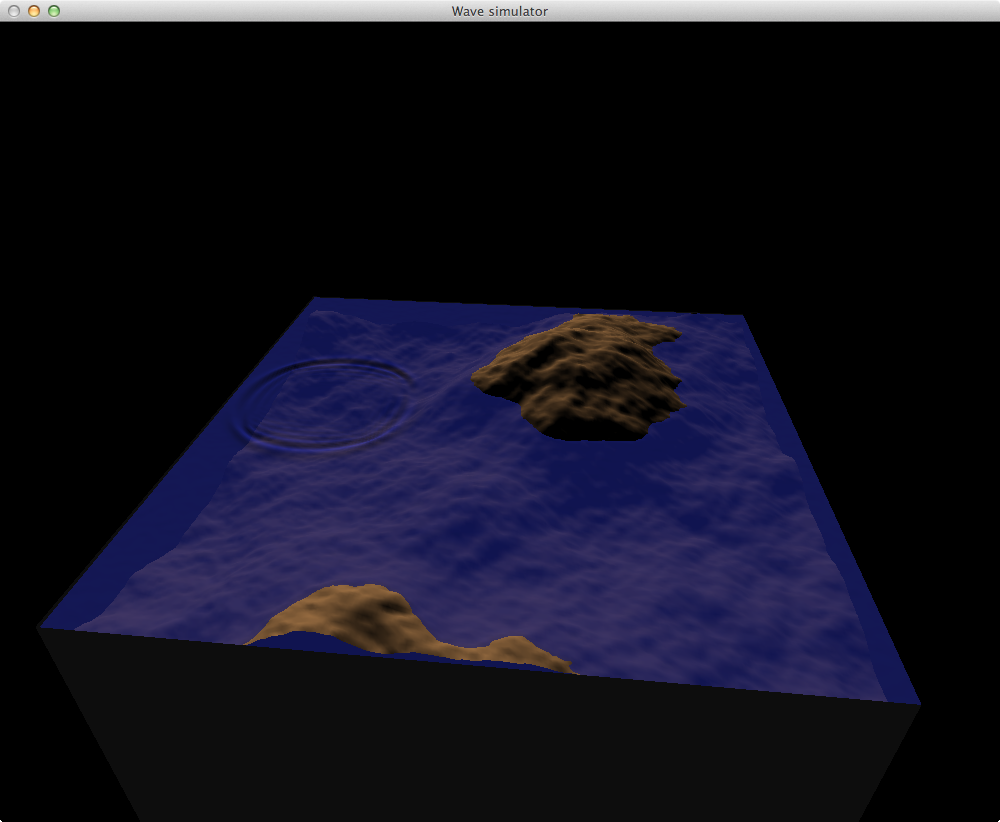
\includegraphics[width=13cm]{ogl1.png}
\caption{Beautiful wave in a realistic wave simulator}
\label{fig:ogl1}
\end{figure}

\begin{figure}
\centering
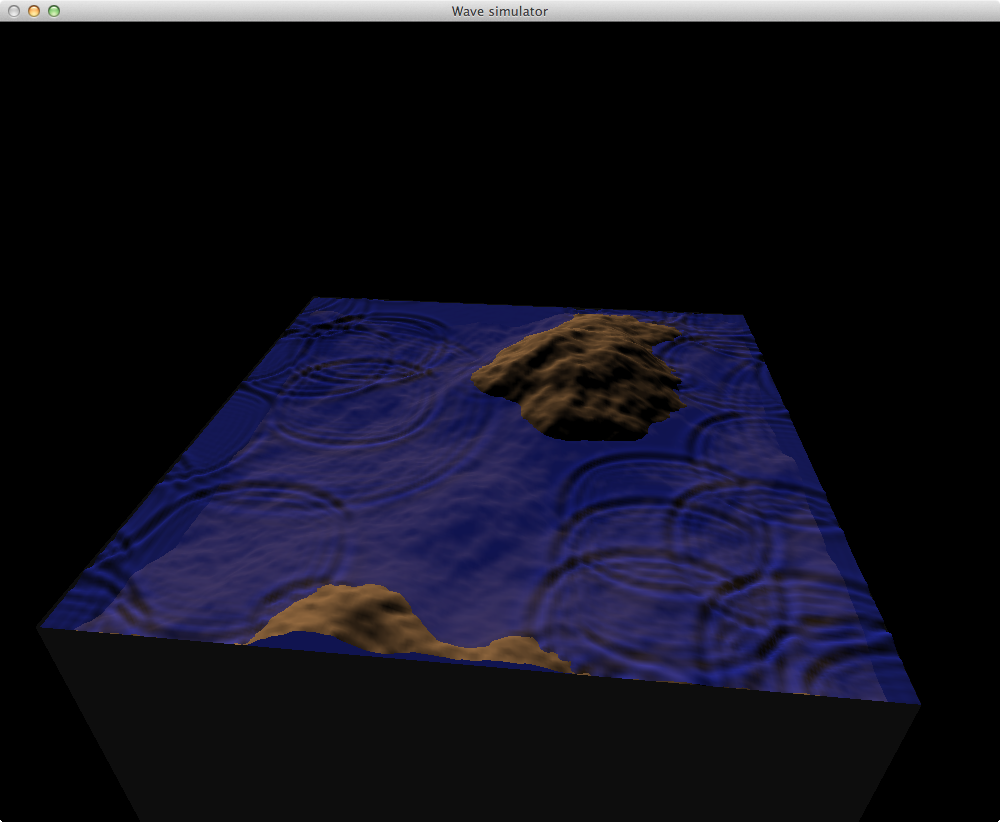
\includegraphics[width=13cm]{ogl2.png}
\caption{Beautiful waves in a realistic wave simulator}
\label{fig:ogl2}
\end{figure}


\end{document}
